\section{Decodability is not dynamical structure}
\label{sec:dissociation}

A probe establishes that a quantity can be read out of a representation. It says nothing about
whether the model's own transition uses or preserves that quantity. We measure the second property
directly, with a statistic on the transition operator: apply one autonomous step at a real encoded
state and ask how much a candidate scalar changes,
\begin{equation}
\rho_{\mathrm{obs}}(C) \;=\;
\frac{\operatorname{median}_t \bigl| C(T(z_t)) - C(z_t) \bigr|}
     {\operatorname{std}_{\mathrm{traj}} C},
\label{eq:rhoobs}
\end{equation}
normalised so it is invariant to the scale of $C$ and comparable across candidates. A value near
zero means the transition preserves $C$; a value near one means a single step moves $C$ by its entire
across-trajectory spread.

\paragraph{A perfect probe identifies a direction the dynamics do not use.}
The sharpest test replaces the label-free search with the answer it is trying to find. We fit a
degree-4 polynomial readout to \emph{true} pendulum energy by ridge regression on the same latent,
then use it to drive the identical correction. It reaches $|\rho|_E = 0.9999$: as a probe it is
essentially perfect.

\begin{figure}[t]
\centering
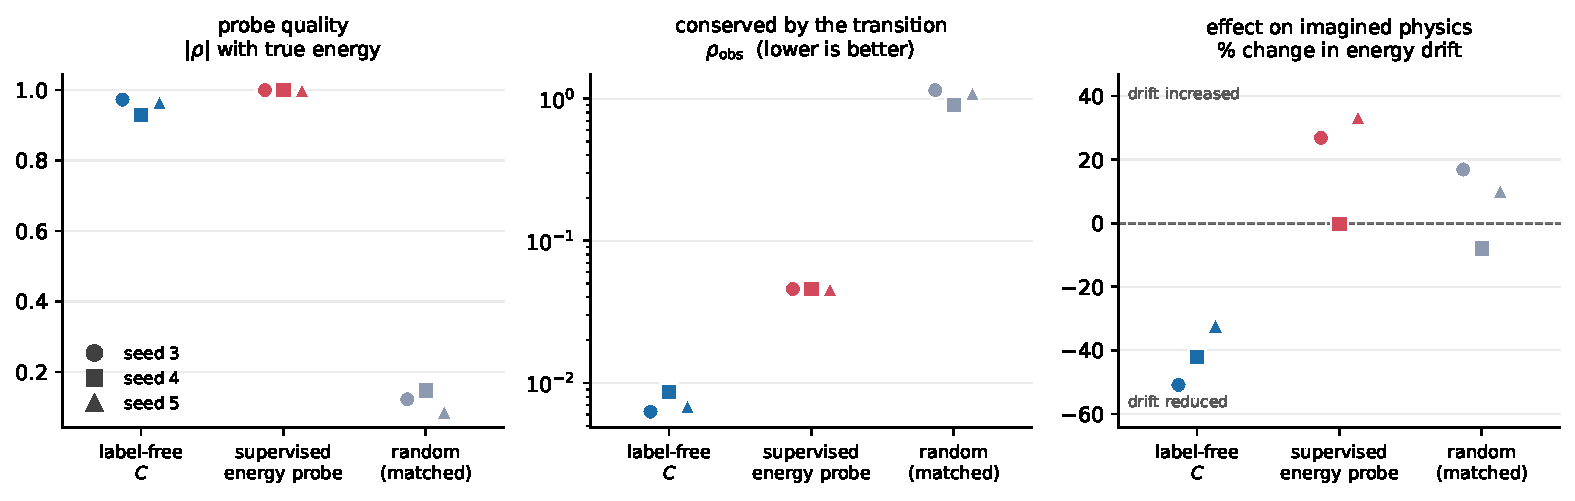
\includegraphics[width=\textwidth]{figures/fig1_probe_vs_operator.pdf}
\caption{A perfect probe is not a conserved quantity. Colour is the constraint; marker is the model
seed (all three shown, never averaged). \textbf{Left:} the supervised probe reads true energy almost
perfectly. \textbf{Centre:} the model's own transition preserves it an order of magnitude worse than
the label-free scalar. \textbf{Right:} acting on it fails to reduce rollout energy drift, while the
label-free scalar cuts drift on every seed. Probe quality and dynamical relevance rank the three
constraints differently.}
\label{fig:probe_vs_operator}
\end{figure}



Figure~\ref{fig:probe_vs_operator} shows the outcome. The supervised
probe tracks energy better than the label-free scalar on every seed, yet is $6.7\times$ less
preserved by the transition --- median $\rho_{\mathrm{obs}}$ of $4.58\times10^{-2}$ against
$6.9\times10^{-3}$, and $5.3$--$7.3\times$ per seed; both hold on 3 of 3 models. It also never repairs the
rollout: its effect on energy drift is $+26.8\%$ and $+33.4\%$ on two models and $-0.3\%$ on the third,
against a median $-42.2\%$ ($32$--$51\%$) reduction from the label-free scalar on all three. A
magnitude-matched random constraint sits at $\rho_{\mathrm{obs}} \approx 1.07$ and changes drift by
$+4.0\%$. The direction that best
predicts the physical variable and the direction the model's dynamics actually respect are not the
same direction.

This also answers the practical objection to a label-free method. The search is not a workaround for
missing labels: it finds something a supervised fit on perfect labels does not, because it optimises
conservation by the transition rather than agreement with the variable.
Section~\ref{sec:mechanism} identifies what it finds, and why fitting true energy cannot find it.

\paragraph{The dissociation is directional, and appears on five further axes.}
In every case we can construct, decodability survives where conservation fails; we have not found the
converse. Table~\ref{tab:axes} collects them. On each row a probe would report success.

\begin{table}[t]
\centering\small
\caption{Decodability is retained while dynamical structure degrades, across five independent axes.
$\rho_{\mathrm{obs}}$ for the trained conservative model in-distribution is $6.3$--$8.7\times10^{-3}$.}
\label{tab:axes}
\begin{tabular}{llcc}
\toprule
axis & contrast & decodability & $\rho_{\mathrm{obs}}$ degradation \\
\midrule
training & untrained network & $|\rho|_E$ up to 0.908 & 74$\times$ \\
state space & outside training energies & free probe 0.999 & 55--267$\times$ \\
architecture & deterministic conv-GRU & $|\rho|_E$ 0.91 (2 of 3 seeds) & 767$\times$ \\
objective & transition never trained & $|\rho|_E$ 0.97 & $\sim$10\,000$\times$ \\
actuation & torque applied & $|\rho|_E$ 0.72--0.88 & balance law absent \\
\bottomrule
\end{tabular}
\end{table}

The out-of-distribution row is cleanest: it holds the model fixed and varies only the region of
state space. Outside the training energy band a freely fitted probe still recovers energy at $0.999$
--- the encoder generalises --- while the transition conserves it $55$--$267\times$ worse, reaching
values indistinguishable from a random constraint. The two properties come apart inside a single
trained model, split by where in state space it is asked.

\paragraph{Under actuation the same split appears against a different law.}
The four axes above vary how well a \emph{conserved} quantity survives; a fifth varies the law
itself. Three further models are trained on the same pendulum under piecewise-constant random torque,
where energy instead obeys $\mathrm{d}E/\mathrm{d}t = \tau\dot\theta$. They demonstrably use their
actions: a 20-step open-loop rollout under the true action sequence beats one under the same actions
shuffled across trajectories, $0.740$--$0.761$ on 3 of 3 seeds. The \emph{unchanged} extraction
recovers an energy-like scalar on every model ($|\rho|_E = 0.72$, $0.88$, $0.86$), yet its motion
under the model's own transition does not follow the balance relation: with the torque known and
$\dot\theta$ from the same decoded readout, the rank correlation with the predicted source term is
$0.041$, $0.076$ and $0.065$, the power term accounts for \textbf{0.31\%} of the variance in
$\Delta C$, and the observed change is $4.5$--$5.4\times$ larger than predicted. A shuffled-power
control is beaten 3 of 3, so the pairing carries something --- almost nothing. The model represents
the quantity and does not implement the relation it obeys, which is also why a correction built on
that scalar confers no control benefit (Section~\ref{sec:limits}): there is no balance structure for
it to enforce.

\paragraph{Whether conservation \emph{alone} predicts the intervention is not established.}
Among candidates matched in energy correlation and spanning five orders of magnitude of conservation,
the rank correlation with repair is $+0.19$, $+0.57$ and $+0.19$ across seeds, with the 95\% interval
excluding zero on \textbf{one of three}. We report this as a negative, and note why the control is
hard: on a system whose transition conserves energy the well-conserved latent directions \emph{are}
the energy-like ones, so a matched band exists only at low decodability and on one seed cannot be
built at all. Appendix~\ref{sec:causal-detail} gives the full analysis. What holds on all three seeds
is that the recovered scalar repairs: $-16.7\%$, $-7.3\%$ and $-6.8\%$.

\paragraph{Where the phenomenon stops.}
Both boundaries above are the same statement seen twice. The invariant is bounded to the
\emph{training distribution}: outside the training energy band a freely fitted probe still recovers
energy at $0.999$ while the transition conserves it $55$--$267\times$ worse, reaching values
indistinguishable from a random constraint. And it is bounded to the \emph{architecture}: on a
deterministic convolutional GRU with no stochastic latent, no KL term and no unimix, identification
transfers on 2 of 3 seeds under both training budgets while conservation transfers on none
($\rho_{\mathrm{obs}}$ $4.83$--$5.55$ against the RSSM's ${\sim}7\times10^{-3}$, a $767\times$ gap;
seven times more open-loop training moved the median from $5.33$ to $5.26$). We are explicit that
this comparison does not isolate architecture --- an open-loop reconstruction term and a
prior--posterior KL are different losses, not the same loss at different strengths --- so the
supportable scope of every claim here is RSSM-like models, in distribution.
